\subsection{Partes} \label{subsec:partes}
En esta sección se presentan los componentes principales del robot, enfocándose en los motores y los eslabones que forman su estructura. Se describe brevemente el papel que desempeña cada uno dentro del sistema, destacando su importancia en el movimiento, la transmisión de fuerzas y el cumplimiento de las tareas asignadas al robot.


\subsubsection{Motores} \label{subsubsec:motores}

En este proyecto se utilizaron tres tipos de motores, cada uno seleccionado de acuerdo con las necesidades específicas de torque, velocidad y precisión. El primero es un motor paso a paso NEMA 17, que de acuerdo con su hoja de datos entrega un torque máximo de 59 N·cm, equivalente a 0.59 N·m. La velocidad máxima considerada para este motor es de 1000 rpm, que corresponde a 2.65 rad/s. Este motor está conectado a una transmisión con una relación de reducción de 8:1, lo que significa que por cada ocho vueltas del motor, la salida da una vuelta. Los motores NEMA 17 son comúnmente usados en impresoras 3D y pequeñas máquinas CNC, debido a su precisión y control fino de pasos.

El segundo motor utilizado es un paso a paso NEMA 23, que tiene un torque máximo de 1.26 N·m y alcanza una velocidad de hasta 1500 rpm, equivalente a 3.98 rad/s. Este motor está acoplado a un reductor con relación 10:1, permitiendo aumentar el torque a costa de reducir la velocidad, lo que lo hace adecuado para aplicaciones que requieren mayor fuerza, como sistemas actuadores más grandes.



Finalmente, se emplea un servo motor de modelo genérico, que ofrece un torque máximo de 350 N·cm (3.5 N·m) y una velocidad aproximada de 60° cada 0.14 segundos, lo cual se traduce a 7.48 rad/s. Este servo está conectado a una transmisión interna de aproximadamente 5:1, la cual permite que el sistema de pinza tenga la precisión y fuerza necesarias para sujetar objetos de forma efectiva. Los servos son ideales para movimientos controlados dentro de un rango limitado, como abrir y cerrar pinzas o mover pequeñas articulaciones.


\subsubsection{Eslabones} \label{subsubsec:eslabones}

Para calcular las propiedades físicas de los eslabones del robot, se utilizaron los datos obtenidos de la configuración de las uniones (joints), en particular las posiciones de origen de cada una. Estas posiciones permiten determinar la longitud aproximada de cada eslabón al observar el desplazamiento relativo entre las articulaciones consecutivas. A partir de estas longitudes, y asumiendo que los eslabones tienen forma cilíndrica con un diámetro aproximado de 2.5 cm, fue posible estimar su volumen. Utilizando aluminio como material base, con una densidad de 2700 kg/m³ —común en aplicaciones de robótica por su ligereza y resistencia—, se calculó una masa aproximada para cada eslabón. Con la masa y la longitud, también se estimó el momento de inercia utilizando la fórmula I = 1/12mL2, correspondiente a un cilindro delgado girando alrededor de su centro.

De esta manera, se obtuvieron los siguientes resultados aproximados para cada eslabón:

El \textbf{eslabón 1}, con una longitud de 0.3991 metros, tiene una masa estimada de 0.85 kg y una inercia de 0.0113 kg·m². \autoref{fig:joint1urdf}.

El \textbf{eslabón 2} tiene una longitud de 0.448 metros, una masa de aproximadamente 0.95 kg y una inercia de 0.016 kg·m². \autoref{fig:joint2urdf}.

El \textbf{eslabón 3} presenta una longitud de 0.2885 metros, con una masa estimada de 0.65 kg y una inercia de 0.0045 kg·m². \autoref{fig:joint3urdf}.

Finalmente, el \textbf{eslabón 4} mide 0.161 metros, con una masa de 0.35 kg y una inercia aproximada de 0.0021 kg·m². \autoref{fig:joint4urdf}.

Estos valores, aunque estimados, ofrecen una base útil para la simulación dinámica del robot y permiten aproximar su comportamiento físico en tareas de control y planificación de movimiento.

\begin{figure}
	\centering
	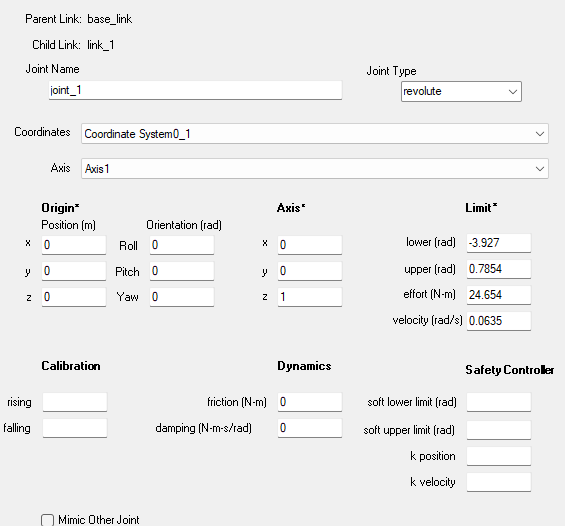
\includegraphics[width=0.3\linewidth]{img/JOINT1URDF}
	\caption{Eslabón 1}
	\label{fig:joint1urdf}
\end{figure}

\begin{figure}
	\centering
	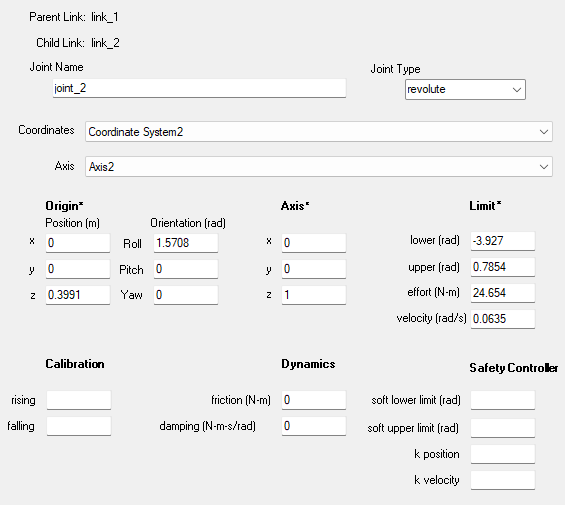
\includegraphics[width=0.3\linewidth]{img/JOINT2URDF}
	\caption{Eslabón 2}
	\label{fig:joint2urdf}
\end{figure}

\begin{figure}
	\centering
	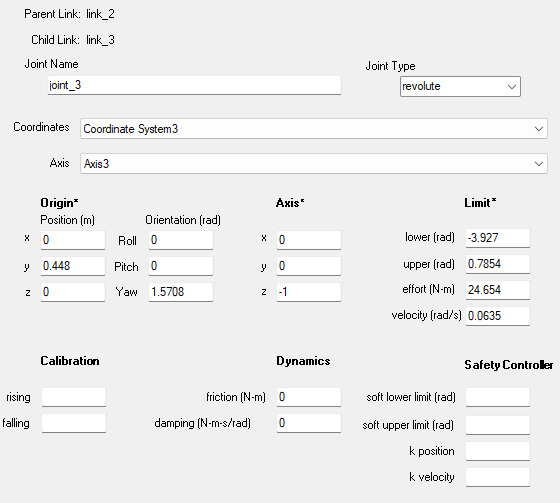
\includegraphics[width=0.3\linewidth]{img/JOINT3URDF}
	\caption{Eslabón 3}
	\label{fig:joint3urdf}
\end{figure}}

\begin{figure}
	\centering
	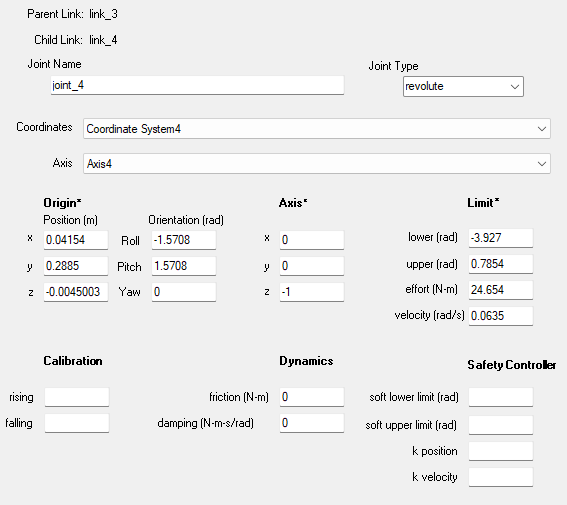
\includegraphics[width=0.3\linewidth]{img/JOINT4URDF}
	\caption{Eslabón 4}
	\label{fig:joint4urdf}
\end{figure}



	





